\section{Greedy Problems}

Greedy problems are problems where the optimal solution can always be developed by, at each opportunity, making the choices that provide the most immediate benefit. In other words, the locally optimal choice is also (part of) the globally optimal choice, in all circumstances. Practically, this just means that at any given step of an algorithm, we can reasonably and reliably make the best choice we can.

For example, a simple greedy problem might look like: we are given a binary search tree (remember that elements larger than a given node are always to the right, as a property of binary search trees), and we must print what the maximum element of this tree is.

The greedy solution to this problem is to always traverse to the right of the tree until we end up at a leaf node. This leaf node is the largest element of the tree, guaranteed by the properties of a binary search tree. In greedy terms, starting from the root of the tree, we will greedy move to the largest child node.

{\centering 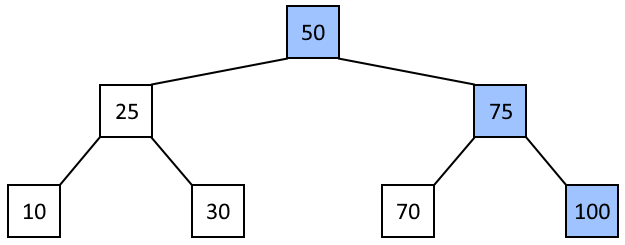
\includegraphics[width=\textwidth]{images/greedy/greedy_tree_1.png}}

In the above example, we can easily verify that 100 is the largest element in the binary search tree.

We can show a similar but slightly modified problem that stops being greedy: we are given a binary tree (that isn't necessarily a binary search tree), and we must print what the maximum element of this tree is.

Here, this is problem is no longer greedy because we can't reliably say that the largest element is always a child of the larger node at each step. Our greedy solution only worked because we could be guaranteed, at each decision, that our locally optimal choice would lead us to the global optimal.

{\centering 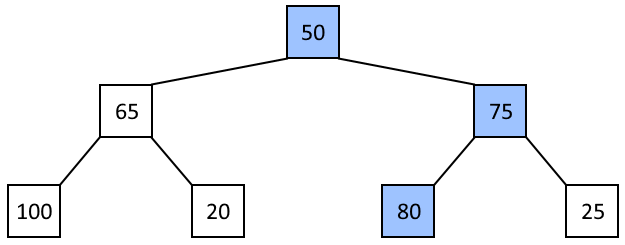
\includegraphics[width=\textwidth]{images/greedy/greedy_tree_2.png}}

While in this case we do greedily take the locally optimal choice at each step, the globally optimal answer involves us taking the locally sub-optimal choice of 65 instead of 75. Because we're not dealing with a binary search tree, we don't have the guarantees we need to greedily approach this problem.

\subsection{Knapsack}

Knapsack problems are those that involve having a knapsack with a maximum capacity $c$, and $n$ items with values $v$ and weights $w$. There are many variants on this problem, but the goal is to put items into the knapsack so that our total value is as high as possible without the total weight exceeding the maximum capacity.

Some knapsack variants are greedy, which we will explore here. Some are not, which won't be covered in depth here, but we will make mention of a few that can't be solved greedily and give reasons why.

\hrulefill

In an unbounded knapsack problem, we can put any amount of an item into the knapsack -- both multiple copies of the same item, and fractional amounts of that item.

The solution in this case is to determine what item has the highest $\frac{v}{w}$ to maximize the value we get for its weight, and then fill the entire knapsack with that.

\hrulefill

In a fractional knapsack problem, we are allowed to put fractional amounts into the knapsack, but we can't put multiple of the same item.

The general concept is the same as before, we greedily use whatever item has the highest $\frac{v}{w}$ because it gives us to most optimal usage of our capacity. This time though, we can't fill our entire knapsack with that one item, and likely have to start using the item with the next highest $\frac{v}{w}$ assuming we still have capacity to spare. We do this until eventually we either run out of items, or we run out of capacity (potentially needing to use a fractional amount of the last item we insert).

\hrulefill

One of the more well known knapsack problems is the 0-1 knapsack problem, where we can only insert an item exactly once, or not at all. In other words, we have to choose for each item whether to include or exclude it.

If we try a greedy approach to this problem, we will quickly find cases where it doesn't work. For example, if our capacity $c$ is $10$, and we're given items with value-weight pairs $\{15,6\},\{8,5\},\{8,5\}$, our greedy approach will take $\{15,6\}$ because $\frac{15}{6} > \frac{8}{5}$, but we can't fill our knapsack with anything more meaning our total value is 15. If we instead go with $\{8,5\}$ we can fill the rest of the knapsack with the other $\{8,5\}$ and end up with a total value of 16.

The issue here being that we can only assume the greedy approach will work if, no matter what choices we make, we can always fill the entire knapsack (assuming we have enough items to fill the entire knapsack). The unbounded knapsack problem and the fractional knapsack problem do this by letting us use fractional amounts of an item. In the 0-1 knapsack problem, we can't make this guarantee, and the locally optimal choice with the highest $\frac{v}{w}$ may not be the globally optimal choice, because another choice may lead to us filling more of the knapsack and ending up with a higher total value.

\subsection{Coin Change}

\subsection{Interval Cover}

In this problem you're given a range $[L,R]$ and a list of intervals $[l,r]$. The task is to determine whether these intervals fully cover the range $[L,R]$.

Let's first consider a non-greedy, recursive approach (formally, a depth-first search approach, that we will describe in a later section). Starting at the leftmost-interval (the interval with the smallest value $l$, even if $r$ is large) that contains $L$, we find every intersection that starts within the range $[l,r]$ (in other words, every overlapping section that's to the right) and then for each we recursively try the same. We will either exhaust all overlapping intervals before we can reach $R$ and know that we can't cover the entire range $[L,R]$, or one of the intervals contains $R$ and know that we do cover the entire range (at which point our algorithm is done).

With recursively considering the leftmost overlapping intervals, we can see in blue what gets considered:

{\centering 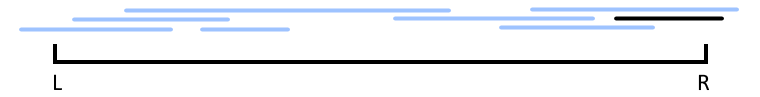
\includegraphics[width=\textwidth]{images/greedy/interval_1.png}}

It's nearly all intervals that get considered, with the only exception being that we find an interval containing $R$ at the end. The above diagram doesn't account for, depending on implementation, that you may end up considering the same interval multiple times as well.

The greedy optimization of this is recognizing that we don't need to check every interval that overlaps, we only need to check the rightmost interval (the overlapping interval with the largest value $r$, \textbf{not} the overlapping interval with the largest value $l$) because it every other interval we might consider is suboptimal to that. This means that we can consider far less intervals.

We can see with the same example as above that we have to check less intervals in total:

{\centering 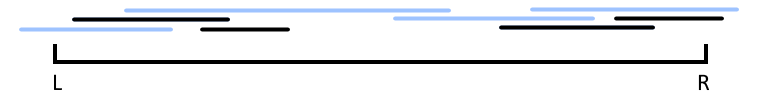
\includegraphics[width=\textwidth]{images/greedy/interval_2.png}}